%% ============================================================
%%  Trade-Side Classification — Beamer Presentation
%%  Compile with: pdflatex presentation.tex  (twice)
%%  Tested on Overleaf (TeX Live 2023)
%% ============================================================
\documentclass[aspectratio=169,10pt]{beamer}

\usetheme{Madrid}
\usecolortheme{beaver}   % dark-red header bars

\usepackage{booktabs}
\usepackage{colortbl}
\usepackage{xcolor}
\usepackage{tikz}
\usepackage{amsmath}
\usepackage{microtype}

%% ── Colours ─────────────────────────────────────────────────
\definecolor{okgreen}{RGB}{0,140,60}
\definecolor{badred}{RGB}{200,30,30}
\definecolor{winrow}{RGB}{220,245,220}
\definecolor{foldA}{RGB}{70,130,180}
\definecolor{foldB}{RGB}{220,80,80}

%% ── Meta ─────────────────────────────────────────────────────
\title{Trade-Side Classification}
\subtitle{Decision Tree vs.\ Classical Baselines}
\author{DreamTeam1 \\ \smallskip
  Michał Brzeziński \quad Benek Kurtyka \quad Krzysztof Nalazek}
\institute{Algorithmic Trading Systems — Final Project}
\date{May 26, 2026}

%% ── Helper: inline code ──────────────────────────────────────
\newcommand{\code}[1]{\texttt{\small #1}}

\begin{document}

% ─────────────────────────────────────────────────────────────
\begin{frame}
  \titlepage
\end{frame}

% ─────────────────────────────────────────────────────────────
\begin{frame}{Outline}
  \tableofcontents
\end{frame}

% ─────────────────────────────────────────────────────────────
\section{Problem \& Data}

\begin{frame}{Problem Statement}
  \begin{block}{What is trade-side classification?}
    Every exchange print has an \textbf{aggressor} — the side that crossed the spread to take
    liquidity.  The public trade feed often omits this label.  We reconstruct it.
  \end{block}

  \medskip
  \begin{columns}[T]
    \column{0.48\textwidth}
    \textbf{Label convention}
    \begin{itemize}
      \item \code{True}  \;= \textbf{sell aggressor} \;(hit the bid)
      \item \code{False} = \textbf{buy aggressor} \quad(lifted the ask)
    \end{itemize}

    \medskip
    \textbf{Why it matters}
    \begin{itemize}
      \item VPIN, Kyle's $\lambda$, order-flow imbalance
      \item Effective spread decomposition
      \item Market-impact models
    \end{itemize}

    \column{0.48\textwidth}
    \begin{exampleblock}{Deliverable}
      \begin{center}
        \code{classify\_side(trades)} $\;\to\;$ \code{pd.Series[bool]}
      \end{center}
      \smallskip
      Input: \code{price}, \code{amount}, \code{time} only\\
      (no order book at inference time)
    \end{exampleblock}
  \end{columns}
\end{frame}

% ─────────────────────────────────────────────────────────────
\begin{frame}{Dataset}
  \begin{columns}[T]
    \column{0.52\textwidth}
    \begin{itemize}
      \item \textbf{Symbols:} WIFUSDT, ZAMAUSDT \;(Binance perps)
      \item \textbf{Data:} trades + L2 order book (10 levels each side)
    \end{itemize}

    \medskip
    \begin{center}
    \begin{tabular}{llrr}
      \toprule
      Split & Date & Trades & Book snaps \\
      \midrule
      Train      & Apr 12 &   41{,}967 &  234{,}390 \\
      Validation & Apr 13 &   47{,}276 &  229{,}094 \\
      \textbf{Test} & \textbf{Apr 14} & \textbf{607{,}949} & \textbf{537{,}684} \\
      \bottomrule
    \end{tabular}
    \end{center}

    \column{0.44\textwidth}
    \begin{block}{Key constraints}
      \begin{itemize}
        \item Order book = \textbf{oracle for training only}
        \item Final function: trades only
        \item Label balance $\approx 52\,\%$ sell / $48\,\%$ buy
        \item Test (Apr 14) touched only at the end
      \end{itemize}
    \end{block}
  \end{columns}
\end{frame}

% ─────────────────────────────────────────────────────────────
\section{Classical Baselines}

\begin{frame}{Baseline 1 — Tick Rule}
  \begin{columns}[T]
    \column{0.50\textwidth}
    \textbf{Algorithm} \quad(trades only — fair baseline)

    \medskip
    \begin{center}
    \begin{tabular}{lc}
      \toprule
      Condition & Label \\
      \midrule
      $\Delta p > 0$ \;(uptick)  & \code{False} — buy \\
      $\Delta p < 0$ \;(downtick)& \code{True}  — sell \\
      $\Delta p = 0$ \;(zero-tick)& carry forward \\
      no prior tick & backward-fill \\
      \bottomrule
    \end{tabular}
    \end{center}

    \medskip
    \textcolor{okgreen}{\textbf{+}} No order book needed \\
    \textcolor{badred}{\textbf{--}} Breaks on flat / high-frequency data

    \column{0.46\textwidth}
    \textbf{Results — ZAMAUSDT}

    \medskip
    \begin{center}
    \begin{tabular}{lcc}
      \toprule
      Date & Accuracy & Macro F1 \\
      \midrule
      Apr 12 (train) & 0.77 & 0.77 \\
      Apr 13 (val)   & 0.80 & 0.80 \\
      \textbf{Apr 14 (test)} & \textbf{0.88} & \textbf{0.88} \\
      \bottomrule
    \end{tabular}
    \end{center}

    \medskip
    \begin{center}
    \begin{tabular}{lrr}
      \multicolumn{3}{c}{\small Confusion matrix — Apr 14}\\
      \toprule
       & pred Buy & pred Sell \\
      \midrule
      true Buy  & 272{,}024 & 38{,}395 \\
      true Sell & 38{,}972  & 258{,}558 \\
      \bottomrule
    \end{tabular}
    \end{center}
  \end{columns}
\end{frame}

% ─────────────────────────────────────────────────────────────
\begin{frame}{Baseline 2 — Quote Rule}
  \begin{columns}[T]
    \column{0.50\textwidth}
    \textbf{Algorithm} \quad(requires order book)

    \medskip
    \begin{center}
    \begin{tabular}{lc}
      \toprule
      Condition & Label \\
      \midrule
      $p < \text{mid}$ & \code{True}  — sell \\
      $p > \text{mid}$ & \code{False} — buy \\
      $p = \text{mid}$ & indeterminate \\
      \bottomrule
    \end{tabular}
    \end{center}

    \smallskip
    $\text{mid} = \dfrac{\text{ask}_0 + \text{bid}_0}{2}$

    \medskip
    \textcolor{okgreen}{\textbf{+}} Highly accurate when price clears mid\\
    \textcolor{badred}{\textbf{--}} Leaves at-the-quote trades unclassified

    \column{0.46\textwidth}
    \textbf{Results — ZAMAUSDT}

    \medskip
    \begin{center}
    \begin{tabular}{lrcc}
      \toprule
      Date & Indet. & Acc. & F1 \\
      \midrule
      Apr 12 & 348 & 0.93 & 0.93 \\
      Apr 13 & 222 & 0.95 & 0.95 \\
      \textbf{Apr 14} & 6{,}528 & \textbf{0.92} & \textbf{0.92} \\
      \bottomrule
    \end{tabular}
    \end{center}

    \medskip
    \begin{center}
    \begin{tabular}{lrr}
      \multicolumn{3}{c}{\small Confusion matrix — Apr 14}\\
      \toprule
       & pred Buy & pred Sell \\
      \midrule
      true Buy  & 285{,}635 & 24{,}784 \\
      true Sell & 26{,}069  & 271{,}461 \\
      \bottomrule
    \end{tabular}
    \end{center}
  \end{columns}
\end{frame}

% ─────────────────────────────────────────────────────────────
\begin{frame}{Baseline 3 — Lee-Ready}
  \begin{columns}[T]
    \column{0.50\textwidth}
    \textbf{Algorithm} \quad(requires order book)

    \medskip
    \begin{center}
    \begin{tabular}{lc}
      \toprule
      Condition & Label \\
      \midrule
      $p < \text{mid}$                        & \code{True}  — sell \\
      $p > \text{mid}$                        & \code{False} — buy  \\
      $p = \text{mid}$ \& downtick            & \code{True}  — sell \\
      $p = \text{mid}$ \& uptick              & \code{False} — buy  \\
      \bottomrule
    \end{tabular}
    \end{center}

    \medskip
    Quote Rule primary; Tick Rule fallback at mid.

    \medskip
    \textcolor{okgreen}{\textbf{+}} Resolves all at-the-quote ambiguities\\
    \textcolor{badred}{\textbf{--}} Still needs the order book

    \column{0.46\textwidth}
    \textbf{Results — ZAMAUSDT}

    \medskip
    \begin{center}
    \begin{tabular}{lrcc}
      \toprule
      Date & Indet. & Acc. & F1 \\
      \midrule
      Apr 12 & 0 & 0.93 & 0.93 \\
      Apr 13 & 4 & 0.95 & 0.95 \\
      \textbf{Apr 14} & 0 & \textbf{0.92} & \textbf{0.92} \\
      \bottomrule
    \end{tabular}
    \end{center}

    \medskip
    \begin{center}
    \begin{tabular}{lrr}
      \multicolumn{3}{c}{\small Confusion matrix — Apr 14}\\
      \toprule
       & pred Buy & pred Sell \\
      \midrule
      true Buy  & 285{,}635 & 24{,}784 \\
      true Sell & 26{,}069  & 271{,}461 \\
      \bottomrule
    \end{tabular}
    \end{center}
  \end{columns}
\end{frame}

% ─────────────────────────────────────────────────────────────
\begin{frame}{Baseline Comparison — Test Set (Apr 14, both symbols)}
  \begin{center}
  \begin{tabular}{lcccc}
    \toprule
    \textbf{Method} & \textbf{Accuracy} & \textbf{Bal.\ Acc.} & \textbf{Macro F1} & \textbf{Errors (FP+FN)} \\
    \midrule
    Quote Rule & 0.9164 & 0.9163 & 0.9163 & 50{,}853 \\
    Lee-Ready  & 0.9164 & 0.9163 & 0.9163 & 50{,}853 \\
    Tick Rule  & 0.8727 & 0.8727 & 0.8727 & 77{,}367 \\
    \bottomrule
  \end{tabular}
  \end{center}

  \medskip
  \begin{block}{Key takeaways}
    \begin{itemize}
      \item Quote Rule $\equiv$ Lee-Ready here: at-the-quote trades are rare ($< 1\,\%$)
      \item Tick Rule trails by $\approx 4\,\%$ — price-level information (midpoint) is critical
      \item These are our targets to beat
    \end{itemize}
  \end{block}
\end{frame}

% ─────────────────────────────────────────────────────────────
\section{Decision Tree with Cross-Validation}

\begin{frame}{Feature Engineering}
  \begin{columns}[T]
    \column{0.50\textwidth}
    \textbf{Trade-only features} (24 total)
    \begin{itemize}\setlength\itemsep{1pt}
      \item Tick direction: lags 1–5, forward-filled
      \item Log-returns: horizons 1, 3, 5, 10 trades
      \item Inter-trade gaps: $\Delta t$, $\log(1{+}\Delta t)$
      \item Volume z-score: rolling 10 / 20 / 50 trades
      \item Run-length \& direction of current streak
      \item Price position in recent 20 / 50-trade range
      \item Round-number proximity, \code{log\_price}
    \end{itemize}

    \column{0.46\textwidth}
    \textbf{Midpoint features} (3 extra, from order book)
    \begin{itemize}
      \item \code{mid\_delta}     $= p - \text{mid}$
      \item \code{mid\_abs\_delta} $= |p - \text{mid}|$
      \item \code{mid\_sign}      $= \text{sign}(p - \text{mid})$
    \end{itemize}

    \medskip
    \begin{block}{Note}
      Midpoint features are used in the \emph{notebook comparison only}.
      The deployed \code{classify\_side()} function operates on trades only.
    \end{block}
  \end{columns}
\end{frame}

% ─────────────────────────────────────────────────────────────
\begin{frame}{Tuning via Time-Series Cross-Validation}
  \begin{columns}[T]
    \column{0.50\textwidth}
    \textbf{Why \code{TimeSeriesSplit}?}
    \begin{itemize}
      \item Financial data is temporally ordered
      \item Each CV fold: training window \emph{strictly before} the validation window
      \item Prevents look-ahead leakage into hyperparameter selection
    \end{itemize}

    \medskip
    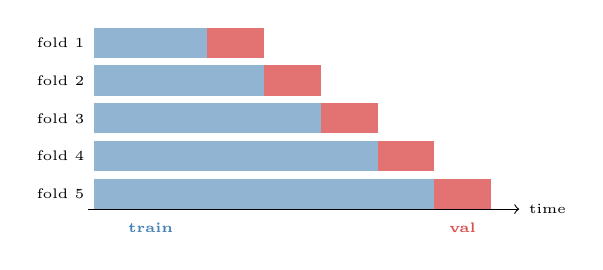
\begin{tikzpicture}[x=0.72cm,y=0.48cm]
      \foreach \f/\ts/\te/\vs/\ve in {
        1/0/2/2/3, 2/0/3/3/4, 3/0/4/4/5, 4/0/5/5/6, 5/0/6/6/7}{
        \fill[foldA!60] (\ts,4-\f) rectangle (\te,4.8-\f);
        \fill[foldB!80] (\vs,4-\f) rectangle (\ve,4.8-\f);
        \node[left,font=\tiny] at (0,4.4-\f) {fold \f};
      }
      \node[font=\tiny,foldA] at (1.0,-1.5) {\textbf{train}};
      \node[font=\tiny,foldB] at (6.5,-1.5) {\textbf{val}};
      \draw[->] (-0.1,-1.0) -- (7.5,-1.0) node[right,font=\tiny]{time};
    \end{tikzpicture}

    \column{0.46\textwidth}
    \textbf{Setup}
    \begin{itemize}
      \item \code{TimeSeriesSplit(n\_splits=5)}
      \item Combined train+val: Apr 12–13 (89{,}243 rows)
      \item \code{Pipeline(SimpleImputer → DT)} \\
            imputer fit on fold train only
      \item Scoring: \code{balanced\_accuracy}
    \end{itemize}

    \medskip
    \textbf{Grid} (216 combinations × 5 folds = 1{,}080 fits)
    \begin{center}
    \begin{tabular}{ll}
      \toprule
      Parameter & Values \\
      \midrule
      \code{max\_depth}           & 4, 6, 8 \\
      \code{min\_samples\_leaf}   & 20, 50, 100 \\
      \code{min\_samples\_split}  & 50, 150 \\
      \code{criterion}            & gini, log\_loss \\
      \code{class\_weight}        & None, balanced \\
      \code{ccp\_alpha}           & 0, 1e-4, 1e-3 \\
      \bottomrule
    \end{tabular}
    \end{center}
  \end{columns}
\end{frame}

% ─────────────────────────────────────────────────────────────
\begin{frame}{CV Results \& Best Parameters}
  \begin{columns}[T]
    \column{0.50\textwidth}
    \begin{block}{Best CV score}
      \textbf{Balanced accuracy = 94.42\%} \\
      (averaged over 5 time-series folds)
    \end{block}

    \medskip
    \textbf{Best parameters:}
    \begin{center}
    \begin{tabular}{ll}
      \toprule
      Parameter & Value \\
      \midrule
      \code{max\_depth}          & 6 \\
      \code{min\_samples\_leaf}  & 20 \\
      \code{min\_samples\_split} & 50 \\
      \code{criterion}           & gini \\
      \code{class\_weight}       & balanced \\
      \code{ccp\_alpha}          & 0.0 \\
      \bottomrule
    \end{tabular}
    \end{center}

    \column{0.46\textwidth}
    \textbf{Top-3 CV candidates}
    \begin{center}
    \begin{tabular}{cccc}
      \toprule
      Rank & depth & weight & CV bal.\ acc \\
      \midrule
      1 & 6 & balanced & 0.9442 \\
      2 & 6 & balanced & 0.9441 \\
      3 & 6 & balanced & 0.9441 \\
      \bottomrule
    \end{tabular}
    \end{center}

    \medskip
    Stable top-3 confirms \code{max\_depth=6} is robustly optimal. \\[0.5em]
    \textbf{Final model:} refit once on full train+val (Apr 12–13), threshold = 0.5.
  \end{columns}
\end{frame}

% ─────────────────────────────────────────────────────────────
\begin{frame}{Feature Importance — What the Tree Learned}
  \begin{columns}[T]
    \column{0.48\textwidth}
    \begin{center}
    \begin{tabular}{lr}
      \toprule
      Feature & Importance \\
      \midrule
      \code{mid\_sign}      & 95.23\,\% \\
      \code{mid\_abs\_delta}& \;1.42\,\% \\
      \code{mid\_delta}     & \;1.12\,\% \\
      \code{ret\_3}         & \;0.49\,\% \\
      \code{log\_amount}    & \;0.32\,\% \\
      \code{tick\_rule\_side}& \;0.25\,\% \\
      others                & \;1.17\,\% \\
      \bottomrule
    \end{tabular}
    \end{center}

    \column{0.48\textwidth}
    \begin{alertblock}{Insight}
      The tree \textbf{rediscovers the Quote Rule} from data: \\
      \code{mid\_sign} $= \text{sign}(p - \text{mid})$ accounts for \textbf{95\,\%} of importance.
    \end{alertblock}

    \medskip
    The remaining 5\,\% is split among magnitude of departure from mid,
    short-term returns, and volume — these capture edge cases where
    the sign alone is ambiguous.
  \end{columns}
\end{frame}

% ─────────────────────────────────────────────────────────────
\begin{frame}{Final Test Results — Decision Tree vs.\ Baselines}
  \begin{center}
  \begin{tabular}{lcccc}
    \toprule
    \textbf{Model} & \textbf{Accuracy} & \textbf{Bal.\ Acc.} & \textbf{Macro F1} & \textbf{Errors (FP+FN)} \\
    \midrule
    \rowcolor{winrow}
    \textbf{Decision Tree (CV)} & \textbf{0.9220} & \textbf{0.9220} & \textbf{0.9220} & \textbf{47{,}393} \\
    Quote Rule & 0.9164 & 0.9163 & 0.9163 & 50{,}853 \\
    Lee-Ready  & 0.9164 & 0.9163 & 0.9163 & 50{,}853 \\
    Tick Rule  & 0.8727 & 0.8727 & 0.8727 & 77{,}367 \\
    \bottomrule
  \end{tabular}
  \end{center}

  \medskip
  \begin{columns}
    \column{0.48\textwidth}
    \begin{alertblock}{DT beats all 3 baselines}
      vs.\ Quote Rule / Lee-Ready: $-3{,}460$ fewer errors\\
      vs.\ Tick Rule: $-29{,}974$ fewer errors
    \end{alertblock}

    \column{0.48\textwidth}
    \begin{exampleblock}{Improvement}
      \begin{tabular}{ll}
        vs.\ Quote Rule: & $+0.57\%$ bal.\ acc. \\
        vs.\ Lee-Ready:  & $+0.57\%$ bal.\ acc. \\
        vs.\ Tick Rule:  & $+4.94\%$ bal.\ acc. \\
      \end{tabular}
    \end{exampleblock}
  \end{columns}
\end{frame}

% ─────────────────────────────────────────────────────────────
\begin{frame}{Confusion Matrices — Test Set (Apr 14, both symbols)}
  \begin{columns}
    \column{0.25\textwidth}
    \begin{center}
    \textbf{Tick Rule}\\[0.4em]
    {\small
    \begin{tabular}{lrr}
      \toprule
       & pBuy & pSell \\
      \midrule
      tBuy  & 272k & 38k \\
      tSell & 39k  & 259k \\
      \bottomrule
    \end{tabular}}
    \end{center}

    \column{0.25\textwidth}
    \begin{center}
    \textbf{Quote Rule}\\[0.4em]
    {\small
    \begin{tabular}{lrr}
      \toprule
       & pBuy & pSell \\
      \midrule
      tBuy  & 286k & 25k \\
      tSell & 26k  & 271k \\
      \bottomrule
    \end{tabular}}
    \end{center}

    \column{0.25\textwidth}
    \begin{center}
    \textbf{Lee-Ready}\\[0.4em]
    {\small
    \begin{tabular}{lrr}
      \toprule
       & pBuy & pSell \\
      \midrule
      tBuy  & 286k & 25k \\
      tSell & 26k  & 271k \\
      \bottomrule
    \end{tabular}}
    \end{center}

    \column{0.25\textwidth}
    \begin{center}
    \textbf{\textcolor{okgreen}{Decision Tree}}\\[0.4em]
    {\small
    \begin{tabular}{lrr}
      \toprule
       & pBuy & pSell \\
      \midrule
      tBuy  & 287k & 24k \\
      \rowcolor{winrow}
      tSell & \textbf{24k}  & \textbf{274k} \\
      \bottomrule
    \end{tabular}}
    \end{center}
  \end{columns}

  \bigskip
  \begin{center}
  \textbf{Key advantage:} DT reduces missed sell aggressors (FN) from 26{,}069 to 23{,}530
  — the largest per-class gain over Quote Rule / Lee-Ready.
  \end{center}
\end{frame}

% ─────────────────────────────────────────────────────────────
\section{Team Models}

\begin{frame}{Gradient Boosting Model — Benek Kurtyka}
  \begin{columns}[T]
    \column{0.50\textwidth}
    \textbf{Approach}
    \begin{itemize}
      \item XGBoost classifier, \textbf{trades only} (no order book)
      \item 24 features: tick direction, returns, volume, streaks
      \item 150 estimators, \code{max\_depth=3}, \code{lr=0.03}
      \item Tuned on validation split (Apr 13)
    \end{itemize}

    \medskip
    \textbf{Results — Test Set (Apr 14)}
    \begin{center}
    \begin{tabular}{lc}
      \toprule
      Metric & Value \\
      \midrule
      Accuracy       & 0.8671 \\
      Balanced Acc.  & 0.8666 \\
      Macro F1       & 0.8668 \\
      Buy F1         & 0.8725 \\
      Sell F1        & 0.8612 \\
      Errors (FP+FN) & 80{,}806 \\
      \bottomrule
    \end{tabular}
    \end{center}

    \column{0.46\textwidth}
    \textbf{Confusion Matrix — Test Set}
    \begin{center}
    \begin{tabular}{lrr}
      \toprule
       & pred Buy & pred Sell \\
      \midrule
      true Buy  & 276{,}517 & 33{,}902 \\
      true Sell & 46{,}904  & 250{,}626 \\
      \bottomrule
    \end{tabular}
    \end{center}

    \medskip
    \textbf{Top feature importances}
    \begin{center}
    \begin{tabular}{lr}
      \toprule
      Feature & Importance \\
      \midrule
      \code{run\_dir}     & 44.25\,\% \\
      \code{tick\_ff}     & 31.49\,\% \\
      \code{pct\_range\_20} & \;3.23\,\% \\
      \code{log\_dt\_s}   & \;1.93\,\% \\
      \code{log\_price}   & \;1.73\,\% \\
      \bottomrule
    \end{tabular}
    \end{center}

    \smallskip
    {\small \textcolor{badred}{Trades-only model — no midpoint access}}
  \end{columns}
\end{frame}

% ─────────────────────────────────────────────────────────────
\begin{frame}{Sequence Model (LSTM) — Krzysztof Nalazek}
  \begin{columns}[T]
    \column{0.50\textwidth}
    \textbf{Approach}
    \begin{itemize}
      \item Causal LSTM, \textbf{trades only} (no order book)
      \item Window: last 32 trades per prediction
      \item 16 relative features (no absolute-price inputs)
      \item Pooled training on both symbols
    \end{itemize}

    \medskip
    \textbf{Results — Test Set (Apr 14)}
    \begin{center}
    \begin{tabular}{lc}
      \toprule
      Metric & Value \\
      \midrule
      Accuracy       & 0.8553 \\
      Balanced Acc.  & 0.8555 \\
      Macro F1       & 0.8553 \\
      Buy F1         & 0.8564 \\
      Sell F1        & 0.8542 \\
      Errors (FP+FN) & 87{,}975 \\
      \bottomrule
    \end{tabular}
    \end{center}

    \column{0.46\textwidth}
    \textbf{Confusion Matrix — Test Set}
    \begin{center}
    \begin{tabular}{lrr}
      \toprule
       & pred Buy & pred Sell \\
      \midrule
      true Buy  & 262{,}287 & 48{,}132 \\
      true Sell & 39{,}843  & 257{,}687 \\
      \bottomrule
    \end{tabular}
    \end{center}

    \medskip
    \begin{block}{Architecture}
      \begin{itemize}
        \item 2-layer LSTM, hidden size 64
        \item MLP head: $64 \to 32 \to 1$ (sigmoid)
        \item BCEWithLogitsLoss, Adam, patience = 5
      \end{itemize}
    \end{block}

    \smallskip
    {\small \textcolor{badred}{Trades-only model — no midpoint access}}
  \end{columns}
\end{frame}

% ─────────────────────────────────────────────────────────────
\begin{frame}{Full Model Comparison — Test Set (Apr 14, both symbols)}
  \begin{center}
  \renewcommand{\arraystretch}{1.15}
  \begin{tabular}{llcccc}
    \toprule
    \textbf{Model} & \textbf{Features} & \textbf{Accuracy} & \textbf{Bal.\ Acc.} & \textbf{Macro F1} & \textbf{Errors} \\
    \midrule
    \rowcolor{winrow}
    \textbf{Decision Tree (CV)} & book+trades & \textbf{0.9220} & \textbf{0.9220} & \textbf{0.9220} & \textbf{47{,}393} \\
    Quote Rule  & book & 0.9164 & 0.9163 & 0.9163 & 50{,}853 \\
    Lee-Ready   & book & 0.9164 & 0.9163 & 0.9163 & 50{,}853 \\
    Tick Rule   & trades & 0.8727 & 0.8727 & 0.8727 & 77{,}367 \\
    GBM (XGBoost) & trades & 0.8671 & 0.8666 & 0.8668 & 80{,}806 \\
    LSTM (Sequence) & trades & 0.8553 & 0.8555 & 0.8553 & 87{,}975 \\
    \bottomrule
  \end{tabular}
  \end{center}

  \smallskip
  \begin{columns}
    \column{0.54\textwidth}
    \begin{alertblock}{Decision Tree beats all 3 baselines}
      Only model with access to midpoint signal —
      fair comparison against Quote Rule \& Lee-Ready (also use order book).
    \end{alertblock}

    \column{0.42\textwidth}
    \begin{block}{Trades-only models}
      GBM and LSTM operate without the order book.
      Their natural reference is \textbf{Tick Rule} (87.3\%).
    \end{block}
  \end{columns}
\end{frame}

% ─────────────────────────────────────────────────────────────
\section{Conclusion}

\begin{frame}{Summary}
  \begin{columns}[T]
    \column{0.48\textwidth}
    \begin{block}{Decision Tree — beats all 3 baselines}
      \begin{tabular}{ll}
        vs.\ Tick Rule:   & $+4.94\%$ acc, $-29{,}974$ err \\
        vs.\ Quote Rule:  & $+0.57\%$ acc, $-3{,}460$ err \\
        vs.\ Lee-Ready:   & $+0.57\%$ acc, $-3{,}460$ err \\
      \end{tabular}\\[0.4em]
      {\small \textit{Uses midpoint features — fair vs.\ oracle baselines}}
    \end{block}

    \medskip
    \begin{block}{GBM \& LSTM — trades-only}
      \begin{tabular}{ll}
        GBM:  & 86.71\% acc, 80{,}806 errors \\
        LSTM: & 85.53\% acc, 87{,}975 errors \\
      \end{tabular}\\[0.4em]
      {\small \textit{Reference: Tick Rule = 87.27\% (also trades-only)}}
    \end{block}

    \column{0.48\textwidth}
    \textbf{Key findings}
    \begin{itemize}
      \item DT rediscovers Quote Rule from data \\
            (\code{mid\_sign} = 95\,\% importance)
      \item \code{TimeSeriesSplit} CV prevents look-ahead leakage
      \item \code{Pipeline} prevents imputation leakage per fold
      \item Without midpoint, learned models roughly match Tick Rule
    \end{itemize}

    \medskip
    \textbf{Notebooks}
    \begin{itemize}\setlength\itemsep{0pt}
      \item[\small$\bullet$] \code{tick\_rule.ipynb}
      \item[\small$\bullet$] \code{quote\_rule.ipynb}
      \item[\small$\bullet$] \code{lee\_ready.ipynb}
      \item[\small$\bullet$] \code{03\_compare\_models.ipynb}
      \item[\small$\bullet$] \code{decision\_tree\_vs\_baselines.ipynb}
    \end{itemize}
  \end{columns}
\end{frame}

\end{document}
